在实际工程中,编译器的选择往往是影响编译速度的关键因素。CMake是一种跨平台的编译工具,它可以用来管理工程的构建,自动生成makefile或project文件,并提供方便的接口来调用编译器、链接器等工具。

\subsection{C++的编译过程}

C++的编译过程可以分为以下几个步骤:

\begin{enumerate}
    \item \textbf{预处理}(Preprocessing):预处理器会对源代码进行预处理,将所有的宏定义、条件编译等操作展开,生成一个新的源文件。
    \item \textbf{编译}(Compilation):编译器会将预处理后的源文件编译成汇编语言。
    \item \textbf{汇编}(Assemble):汇编器会将汇编语言代码转换成机器语言。
    \item \textbf{链接}(Linking):链接器会将多个目标文件和库文件链接成一个可执行文件。
\end{enumerate}

\begin{figure}[H]
    \centering
    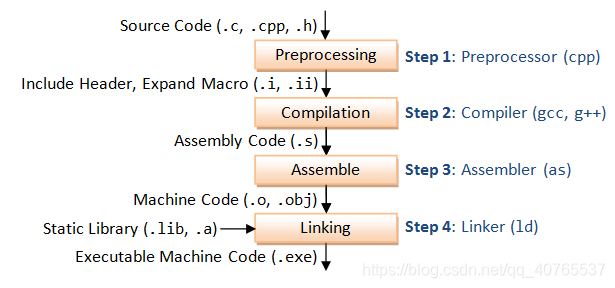
\includegraphics[width=0.7\textwidth]{编译流程.png}
    \caption{C++编译过程} % 图片标题
    \label{fig:编译} % 图片标签,用于引用
\end{figure}

\textbf{预编译}:
预编译器会对源代码进行预处理,将所有的宏定义、条件编译等操作展开,生成一个新的源文件。
预编译器的作用主要是对源代码进行预处理,以便于编译器进行编译。
比如说,对于一个头文件引用$\#include<iostream>$,预编译器会将其展开为头文件的源代码,
生成一个新的源文件,然后再进行编译。对于头文件,预编译器只会进行一次,而对于源文件,
预编译器会在每个源文件编译前进行一次。在代码中的宏定义$\#define$会在预编译时进行字符串替换,
而条件编译$\#if$则会根据条件是否成立来决定是否展开代码。
只有理解了这些,才能真正理解宏和条件编译的作用。

在C/C++中有一些预定义的宏,可以拿来直接用,如:
\begin{tcode}
__FUNTION__  获取当前函数名 
__LINE__ 获取当前代码行号 
__FILE__ 获取当前文件名 
__DATE__ 获取当前日期 
__TIME__ 获取当前时间
__STDC_VERSION__  获取当前编译器的版本
\end{tcode}

\textbf{编译}:
编译器会将预处理后的源文件编译成汇编语言。
编译阶段进行语法分析、词法分析和语义分析,并且将代码优化后产生相应的汇编代码文件(ASCLL文件),
即.s 文件。这个过程是整个程序构建的核心部分,也是最复杂的部分之一。

\textbf{汇编}:
通过不同平台(Windows、Linux)的汇编器将汇编代码翻译成机器码,即生成二进制可重定向文件(.o)。
任何一个源文件在进行编译阶段的时候会去产生\textbf{符号表},符号表中存放的就是程序所产生的符号
(例如:函数名,变量名等),我们的编译阶段是不会去给符号分配正确的地址。这些\textbf{符号}都没有被分配地址,
因此.o文件没有经过链接是无法执行的。

\textbf{链接}:
链接器会将多个目标文件和库文件链接成一个可执行文件。
链接器的作用是将多个目标文件和库文件链接成一个可执行文件,这个过程会将符号表中的符号分配正确的地址,
并将各个目标文件中的代码和数据合并到一个可执行文件中。
简单来说,\textbf{连接就是将符号和数据进行整合,最终得到一个可以指定的文件。}

链接有两种方式:\textbf{静态链接}和\textbf{动态链接}。
相对应的,这两种链接方式所对应的库就称为\textbf{静态库}和\textbf{动态库}。

\textbf{静态库}:
静态库是编译好的目标文件,在链接时会被直接链接到可执行文件中。
静态库的优点是编译速度快,缺点是可执行文件体积大,因为它包含了所有程序需要的目标文件。

\textbf{动态库}:
动态库是运行时加载的库,在程序运行时才被加载到内存中。
动态库的优点是可执行文件体积小,缺点是运行速度慢,因为它需要在运行时加载。

\subsection{CMake}
从上面的介绍中,可以看出,编译过程是十分复杂的,错误的编译方式可能会导致编译失败,或者编译的程序无法正确运行。
为了告诉编译器如何编译我们的程序,工程师们开发了$makefile$,它是一种描述编译过程的脚本文件。
$makefile$的优点是简单易懂,缺点是不够灵活,工程师需要写大量的$makefile$,并且需要手动管理。
在这种困境下,CMake应运而生。

\textbf{CMake}是一种跨平台的编译工具,它可以用来管理工程的构建,自动生成$makefile$或$project$文件,
并提供方便的接口来调用编译器、链接器等工具。$CMake$的优点是简单易用,它会根据工程的结构自动生成$makefile$,
并且可以自动检测编译器、库的安装路径,使得工程师只需要关注工程的源代码即可。

CMake的使用十分简单,只需要在工程的根目录下创建一个$CMakeLists.txt$文件,然后在其中写入编译指令即可。
主要的工作内容有:

\begin{enumerate}
    \item \textbf{项目配置}:确定工程的名称、版本、作者、编译器、编译器版本、编译类型等。
    \item \textbf{添加文件}:添加工程需要编译的源文件和头文件,查找依赖包,并将其加入编译列表。
    \item \textbf{编译}:使用CMake提供的接口编译工程,生成重定向文件和库文件。
    \item \textbf{连接}:将重定向文件和库文件链接成可执行文件。
    \item \textbf{安装}:将可执行文件安装到指定目录。
\end{enumerate}

下面我们来逐个分析介绍一下CMake的使用方法:

\subsubsection{项目配置}
使用CMake的第一步是配置工程,首先需要创建一个$CMakeLists.txt$。
在$CMakeLists.txt$文件中,
我们需要指定工程的信息,如项目名称、编译器、编译器版本、编译选项等。需要强调的是,
$CMake$本身\textbf{不具有编译功能},它只是用来管理工程的构建,具体来说,是形成一套编译器可以“看懂”的文件
然后编译器根据这些文件进行编译。

常用的命令有:
\begin{tpython}
project(project_name)  # 设置项目名称
cmake_minimum_required(VERSION 2.8)  # 设置CMake的最低版本
set(CMAKE_CXX_COMPILER "g++")  # 设置编译器
set(CMAKE_CXX_FLAGS "-Wall -g")  # 设置编译选项
set(CMAKE_CUDA_COMPILER /usr/local/cuda-11.8/bin/nvcc) # 设置CUDA编译器路径
enable_language(CUDA)  # 启用CUDA语言
\end{tpython}
需要强调的是,$CMake$的指令(括号外)是不区分大小的。但是变量和值(括号内)是大小写\textbf{敏感}的。

后期还会使用到的一些指令:
\begin{tpython}
set(CMAKE_CUDA_COMPILER /usr/local/cuda-11.8/bin/nvcc) # 设置CUDA编译器路径
enable_language(CUDA)  # 启用CUDA语言
\end{tpython}

这里需要特别强调一下$set$指令,它可以设置变量的值,并可以用变量来代替值。
可以使用\textbf{宏}来读取$set$所设置的变量的值,如:
\begin{tpython}
message(STATUS ${CMAKE_CXX_COMPILER})  # 打印编译器路径
\end{tpython}

其中,$CMAKE\_CXX\_COMPILER$是$CMake$预定义的宏,表示编译器的路径,使用$\$\{\}$可以使用宏的值。
$CMake$中所有的配置过程都是在进行\textbf{宏}的配置,这里体现一种$set$两种用法的统一性,我们可以根据自己的需求来设置。

\subsubsection{添加文件}

在$CMakeLists.txt$文件中,我们需要添加工程需要编译的源文件和头文件,查找依赖包,并将其加入编译列表。

常用的命令有:
\begin{tpython}
include_directories(include)  # 添加文件目录
# 添加使用*查找所有的文件,并将其加入变量YOLOV8_SRCS
file(GLOB_RECURSE YOLOV8_SRCS ${PROJECT_SOURCE_DIR}/src/yolov8/*.cpp ) 
link_directories(/usr/local/cuda/lib64) # 添加链接目录
\end{tpython}

除此之外,还可以使用\textbf{find\_package}指令来查找依赖包,并将其加入编译列表。例如:

\begin{tpython}
# 查找OpenCV依赖包
find_package(OpenCV REQUIRED)
\end{tpython}
$REQUIRED$参数表示如果依赖包没有找到,则会报错。

$CMake$还为我们提供了一些逻辑判断指令,如:
\begin{tpython}
set(SAVE_OUTPUT "true") #是否要保存输出
if(SAVE_OUTPUT STREQUAL "true")
    message(STATUS "Save output ON\n")
    add_definitions(-DSAVE_OUTPUT)
else()
    message(STATUS "Save output OFF\n")
endif()
\end{tpython}

通过这些逻辑判断指令,我们可以根据自己的需求来控制编译过程。
并且还可以使用\textbf{if}指令来控制编译选项,
这些指令的加入,丰富了$CMake$的功能,使得工程师可以更加灵活地管理编译过程。

\subsubsection{编译}

在$CMakeLists.txt$文件中,我们可以使用\textbf{add\_executable}指令来编译工程:

\begin{tpython}
add_executable(${PROJECT_NAME} ${YOLOV8_SRCS})  # 编译成重定向/可执行文件
\end{tpython}

在$add\_executable$指令后面,我们需要指定可执行文件名称和需要编译的源文件。
这里可以不写头文件,因为$CMake$会根据我们设置的\textbf{项目文件目录},自动查找头文件。

还可以使用$add\_library$指令来编译库文件:

\begin{tpython}
add_library(${PROJECT_NAME} ${YOLOV8_SRCS})  # 编译成动态库文件
add_library(yolov8 STATIC ${YOLOV8_SRCS})  # 编译成静态库文件
\end{tpython}

\subsubsection{链接}

链接器会将多个目标文件和库文件链接成一个可执行文件。主要使用$target\_link\_libraries$指令来链接:

\begin{tpython}
target_link_libraries(${PROJECT_NAME} ${OpenCV_LIBS})  # 链接依赖库
\end{tpython}

$target\_link\_libraries$指令后面需要指定\textbf{重定向文件名称}和\textbf{依赖库的名称}。

\subsubsection{安装}

$CMake$还提供了$install$指令来安装可执行文件:

\begin{tpython}
install(TARGETS ${PROJECT_NAME} DESTINATION bin)  # 安装可执行文件
\end{tpython}

这里需要指定\textbf{可执行文件名称}和\textbf{安装路径}。

\subsubsection{补充内容}

\textbf{添加文件有两种方式},即全局的和局部的。
命令分别是:
$include\_directories$和$target\_include\_directories$。
局部的指令只对当前目标有效,全局的指令对整个工程有效。

为了方便同学们调试,我们写了一个简单的调试函数:

\begin{tpython}
function(print_var var)
set(value "${${var}}")
string(LENGTH "${value}" value_length)
if(value_length GREATER 0)
    math(EXPR last_index "${value_length} - 1")
    string(SUBSTRING "${value}" ${last_index} ${last_index} last_char)
endif()

if(NOT "${last_char}" STREQUAL "\n")
    set(value "${value}\n")
endif()
message(STATUS "${var}:\n   ${value}")
endfunction()
\end{tpython}

在你的项目中,可以创建一个.cmake文件,然后在CMakeLists.txt中调用:

\begin{tpython}
#导入一些CMake函数
list(APPEND CMAKE_MODULE_PATH "${CMAKE_CURRENT_SOURCE_DIR}/cmake")
include(Function)

print_var(CMAKE_CXX_COMPILER)
print_var(CMAKE_CXX_FLAGS)
print_var(CMAKE_CUDA_COMPILER)
\end{tpython}

\begin{figure}[H]
    \centering
    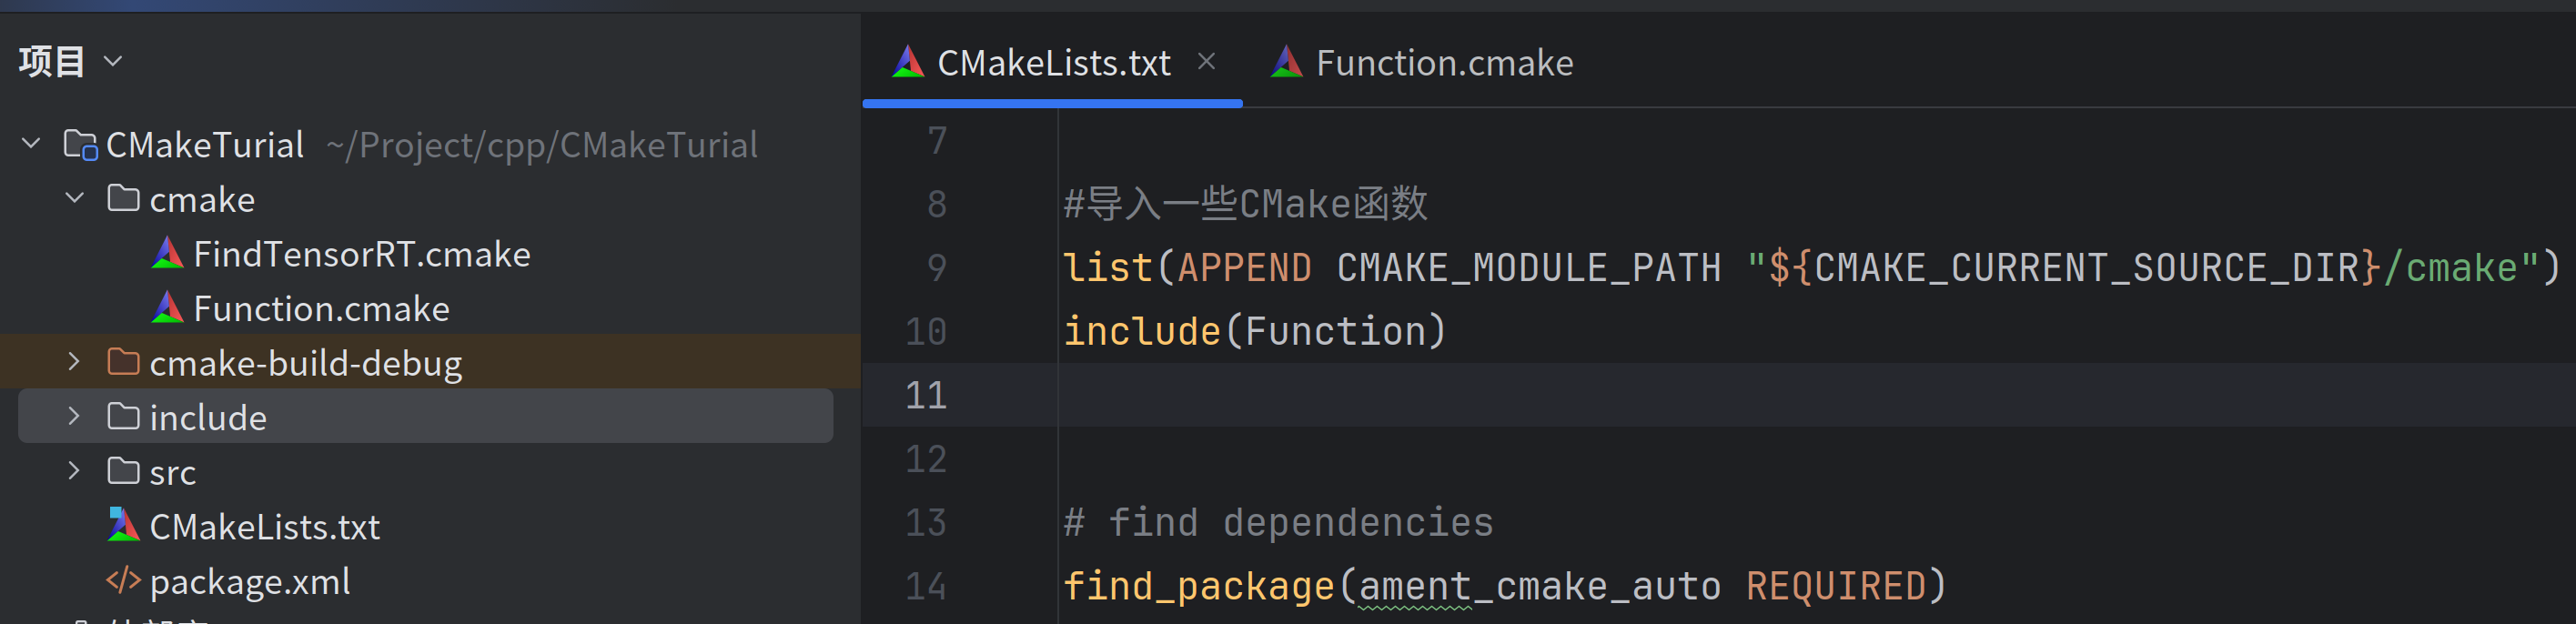
\includegraphics[width=0.7\textwidth]{cmake函数.png}
    \caption{实例项目结构} % 图片标题
    \label{fig:cmakeFunction} % 图片标签,用于引用
\end{figure}

这样,就可以在编译时打印出相关信息,方便调试。

\subsubsection{实例}

下面是一个实例项目的$CMakeLists.txt$文件,请试着读懂它:

\begin{tpython}
cmake_minimum_required(VERSION 3.8)
project(filter)

if(CMAKE_COMPILER_IS_GNUCXX OR CMAKE_CXX_COMPILER_ID MATCHES "Clang")
    add_compile_options(-Wall -Wextra -Wpedantic)
endif()

#导入一些CMake函数
list(APPEND CMAKE_MODULE_PATH "${CMAKE_CURRENT_SOURCE_DIR}/cmake")
include(Function)


# find_package 的高级平替,后面会讲
find_package(ament_cmake_auto REQUIRED)
ament_auto_find_build_dependencies()

###################项目目录设置######################
set(KALMAN_INCLUDE_DIR ${PROJECT_SOURCE_DIR}/include/kalman)
set(KALMAN_SRC_DIR ${PROJECT_SOURCE_DIR}/src/kalman)
set(MLS_INCLUDE_DIR ${PROJECT_SOURCE_DIR}/include/mls)
set(MLS_SRC_DIR ${PROJECT_SOURCE_DIR}/src/mls)
set(LMS_INCLUDE_DIR ${PROJECT_SOURCE_DIR}/include/lms)
set(LMS_SRC_DIR ${PROJECT_SOURCE_DIR}/src/lms)
set(EXEC_INCLUDE_DIR ${PROJECT_SOURCE_DIR}/include/exec)
set(EXEC_SRC_DIR ${PROJECT_SOURCE_DIR}/src/exec)

file(GLOB_RECURSE EXEC_SRCS ${EXEC_SRC_DIR}/*.cpp)
file(GLOB_RECURSE KALMAN_SRCS ${KALMAN_SRC_DIR}/*.cpp)
file(GLOB_RECURSE MLS_SRCS ${MLS_SRC_DIR}/*.cpp)
file(GLOB_RECURSE LMS_SRCS ${LMS_SRC_DIR}/*.cpp)

list(APPEND ALL_INCLUDE
        ${KALMAN_INCLUDE_DIR} ${MLS_INCLUDE_DIR} ${EXEC_INCLUDE_DIR} ${LMS_INCLUDE_DIR}
        ${OpenCV_INCLUDE_DIRS} ${EIGEN3_INCLUDE_DIR})

print_var(ALL_INCLUDE)

print_var(EXEC_SRCS)
print_var(KALMAN_SRCS)
print_var(MLS_SRCS)
print_var(LMS_SRCS)

include_directories(${ALL_INCLUDE})

##############静态库编译##################
add_library(filter_kalman ${KALMAN_SRCS})
add_library(filter_mls ${MLS_SRCS})
add_library(filter_lms ${LMS_SRCS})
list(APPEND FILTER_LIBS
        ${filter_kalman} ${filter_mls} ${filter_lms}
)
print_var(FILTER_LIBS)
############项目编译构建##########################
# add_executable的高级平替,以后会讲
ament_auto_add_executable(filter ${EXEC_SRCS})

target_link_libraries(filter ${OpenCV_LIBS} ${FILTER_LIBS})

# 这里进行项目的安装
if(BUILD_TESTING)
    find_package(ament_lint_auto REQUIRED)
    # the following line skips the linter which checks for copyrights
    # comment the line when a copyright and license is added to all source files
    set(ament_cmake_copyright_FOUND TRUE)
    # the following line skips cpplint (only works in a git repo)
    # comment the line when this package is in a git repo and when
    # a copyright and license is added to all source files
    set(ament_cmake_cpplint_FOUND TRUE)
    ament_lint_auto_find_test_dependencies()
endif()

# 神秘小代码,以后会讲
ament_auto_package()    
\end{tpython}

学了上面的内容,相信你已经可以写出自己的$CMakeLists.txt$文件了。
